\section*{Simulation of SDN networks using the POX controller}
In week 06 experiment, we employ the use of software defined networks (SDN) with the pox controller in a virtualized network environment with mininet.
\subsection*{1. Introduction}
The main topic of the week06 experiment, SDN and openflow , are the new proposal to overcome the nowdays structual problem of internet that it is based on the transfer service end-to-end and protocol stack TCP / IP.

So that current architerture of internet, the intelligence systems are located in the ends of the network with core contains very simple information as we can figured out those IP protocols work in \textbf{week 01, 02 experiment} with wireshark.The nodes of the core network do not provide information about its operation, and it implies that the user get troubled when the network does not work the node does not contain the any information where the error occured in.

The other example of the simple and transparent core with the same reason is a large overhead of manual configuration, debugging, and design new applications. 
We also checked those in the last \textbf{week 02 experiment}, the TCP protocol was used to perform the aforementioned functions. 
That the TCP’s overhead contains the extra offset data area about amount of 1 $\sim$ 2 times compared to the pure socket has.

\subsection*{2. SDN \& Openflow}
To overcome the limitations metioned above, SDN(software defined) and Openflow were introduced. In short those problems in traditional networks are that both the control and data planes are tightly integrated and implementes in the forwarding devices that comprise a network. In this respect SDN is a networking paradigm where the data and control planes are decoupled from one another\footnote{One can think of the control plane as being the netwokrs ‘Brain’, i.e., it is responsible making all decisions, for example, how to forward data, while the data plane is what aactually moves the data.} 

The SDN control plane is implemented by the ‘controller’ and the data plane by ‘switches’. The controller acts as the “Brain” of the network, and send commands(”Rules”) to the switches on how to handle traffic. 
Openflow has emerged as the de facto SDN standard and specifies how the controller and the switches communicate s well as the rules controllers install on switches.

The objectives of this week, we learn the how SDN and its standard, openflows does work as setting the sample scenario with SDN based Hub and L2 learning switch. 

\subsection*{3. Experiment in virtual environment}
\subsubsection*{Why virtual environment?}
Since the experiment in the real network environment it is hard to setting the component we posed to observing their work in given scenario, also can hardly be evaluated, we implement the virtual network environment by using the mininet \& POX controller.  
\subsubsection*{POX controller \& Mininet}
In this network simulation expeiment employing the use of SDN with POX controllers in a virtualized environment with Minitnet in which the results will be evaluated.
\subsection*{4. Simulation of SDN networks using the POX controller}
% \subsubsection*{Simulation Scenario}
The Simulation scenario consists of a single OpenFlow Switches (s1) connected to three hosts (h1, h2, h3).\\
\vspace{-4mm}
\begin{figure}[!h]\centering 
	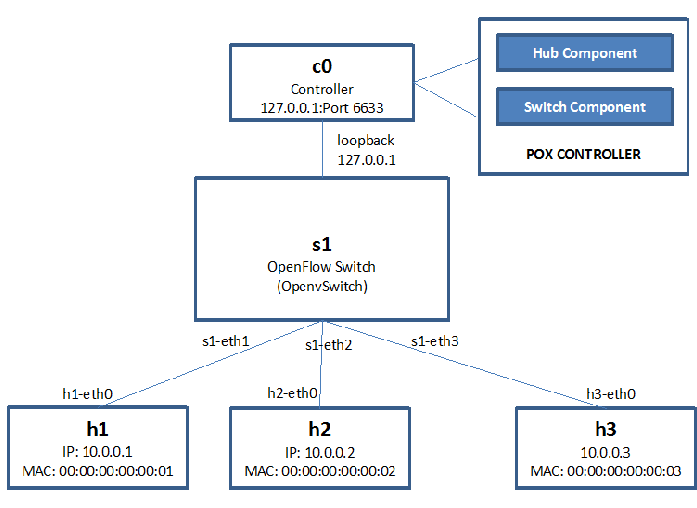
\includegraphics[width=.6\textwidth]{image/week06/0-1.png}
	\caption{\footnotesize 
	Simulation Scenario of topology used in week 06 experiment}
	\vspace{-10pt}
\end{figure}

And there are two ways to implemnt the given scenario topology by mininet. The one is the mentioned in the Experiment lecture material, that command the CLI in bash terminal in ubuntu environment, and the other is writing a custom python code since the mininet is builded by python API and we can easily make the scenario instead of writing a command line by line in bash terminal.\\
We have implemented the basic topology of mininet to be used in Experiments 1, 2, and 3 in the two methods mentioned.
\subsubsection*{mininet CLI}
In the mininet terminal it was used commands of code below to build a topology as shown in Figure 1 :
\begin{center}
    \begin{verbatim}
        sudo mn --topo single,3 --mac --switch ovsk --controller remote
    \end{verbatim}
\end{center}
\vspace{-4mm}
The parameter used in the code are described below (all of those a family of mininet CLI commands, implimented in "./mininet/topo/\_\_main\_\_.py" ):
\begin{itemize}
    \item \textbf{mn} : it starts the CLI mininet in bash terminal.
    \item \textbf{-- topo single,3} : it creates a topology with 3 virtual hosts, each one containing a separated IP address.
    \item \textbf{-- mac} : it sets the MAC address of each host equal to its IP. As a standard the hosts and switches begin at random MAC addresses. This can make it difficult to debug network applications, since each new execution Mininet generates MAC addresses distinct from their hosts and switches. To solve this problem we can use the option --mac where each node has a simple and easy address to read.
    \item \textbf{-- switch ovsk} : it creates a single OpenFlow switch in software (OpenvSwitch) kernel with 3 doors.
    \item \textbf{-- controller remote} : it sets the Openflow switch to connect to a remote contreller.
\end{itemize}
The figure below is the terminal output after we execute the mininet CLI code in bash terminal.\\
\vspace{-4mm}
\begin{figure}[!h]\centering 
	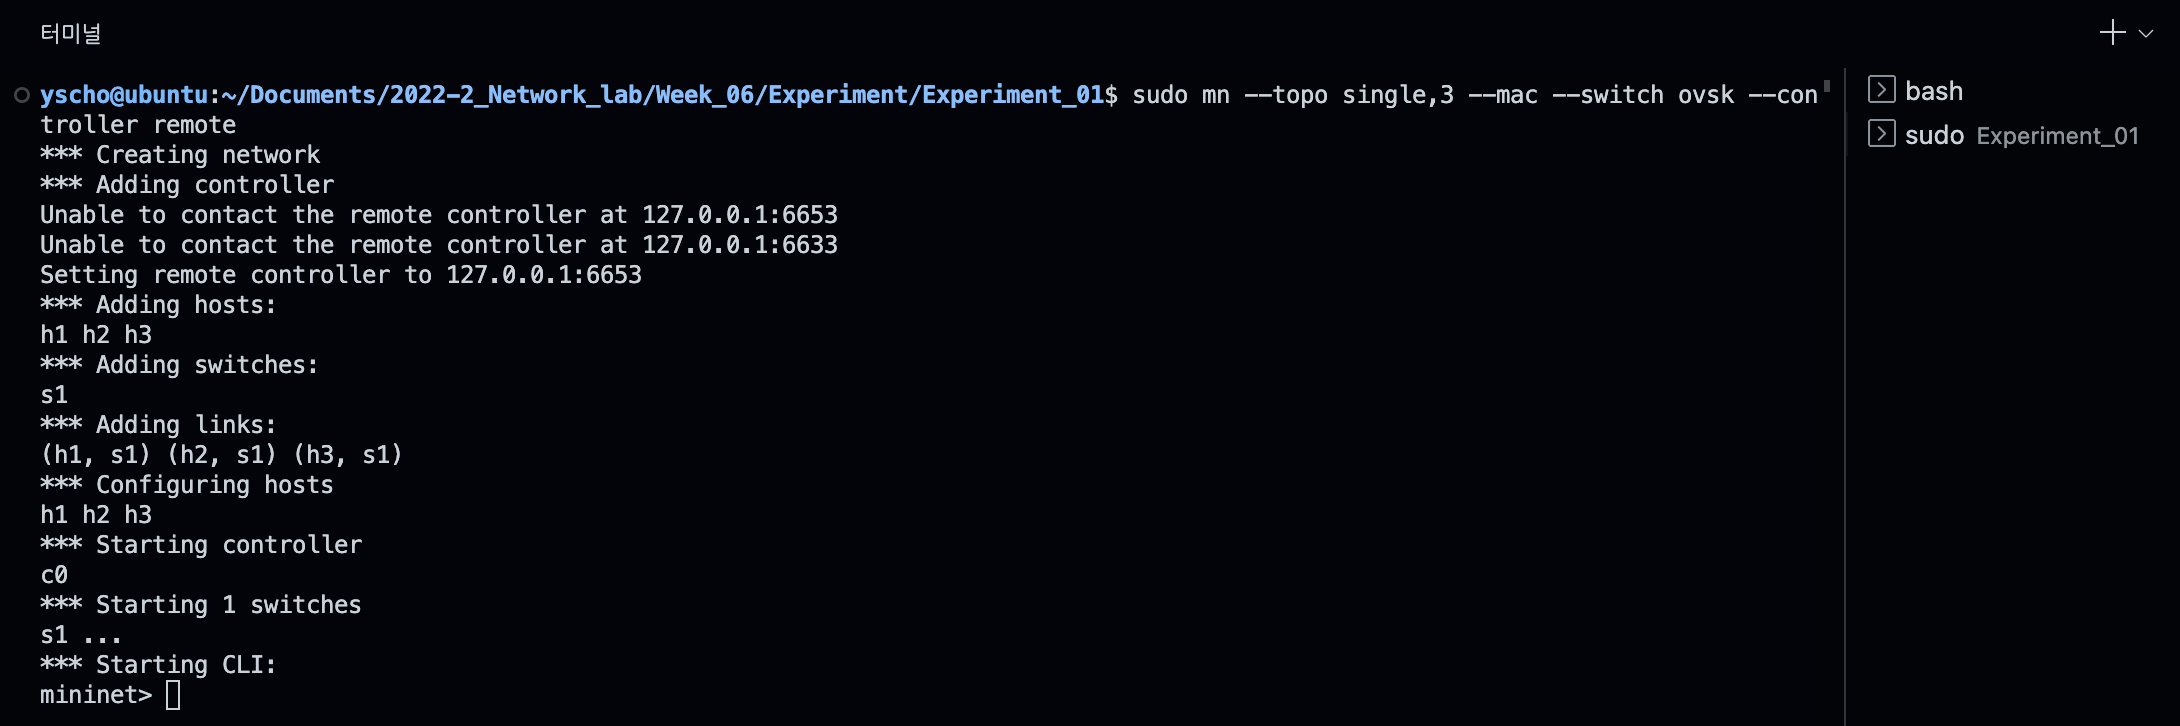
\includegraphics[width=.9\textwidth]{image/week06/1-3-1.png}
	\caption{\footnotesize 
	Terminal out screenshot : After executing the mininet CLI command in bash terminal}
	\vspace{-10pt}
\end{figure}
\vspace{-4mm}
\subsubsection*{mininet python API}
By writting complete mininet scripts in python, it can be esaily cusomized the mn command line tool using —custom options. That all options command in CLI like ‘—topo’, defined as member of dictionary’s keys. 
So as we can use the simple polomorphism of class that implemented in mininet API to build a custom scenario scripts.
The python scripts below just same as the given mininet CLI command.
\begin{listing}[h!]
\inputminted[framerule = 1pt,framesep = 2mm , frame = lines, fontsize=\scriptsize]{python}{./code/week06/basic_topo.py}
\caption{\footnotesize 1 switch and 3 host consturction with mac option that setting the simple IP address automatically}
\end{listing}
\clearpage
The figure below is the terminal output after we execute the custom python topology code in bash terminal.\\
\vspace{-4mm}
\begin{figure}[!h]\centering 
	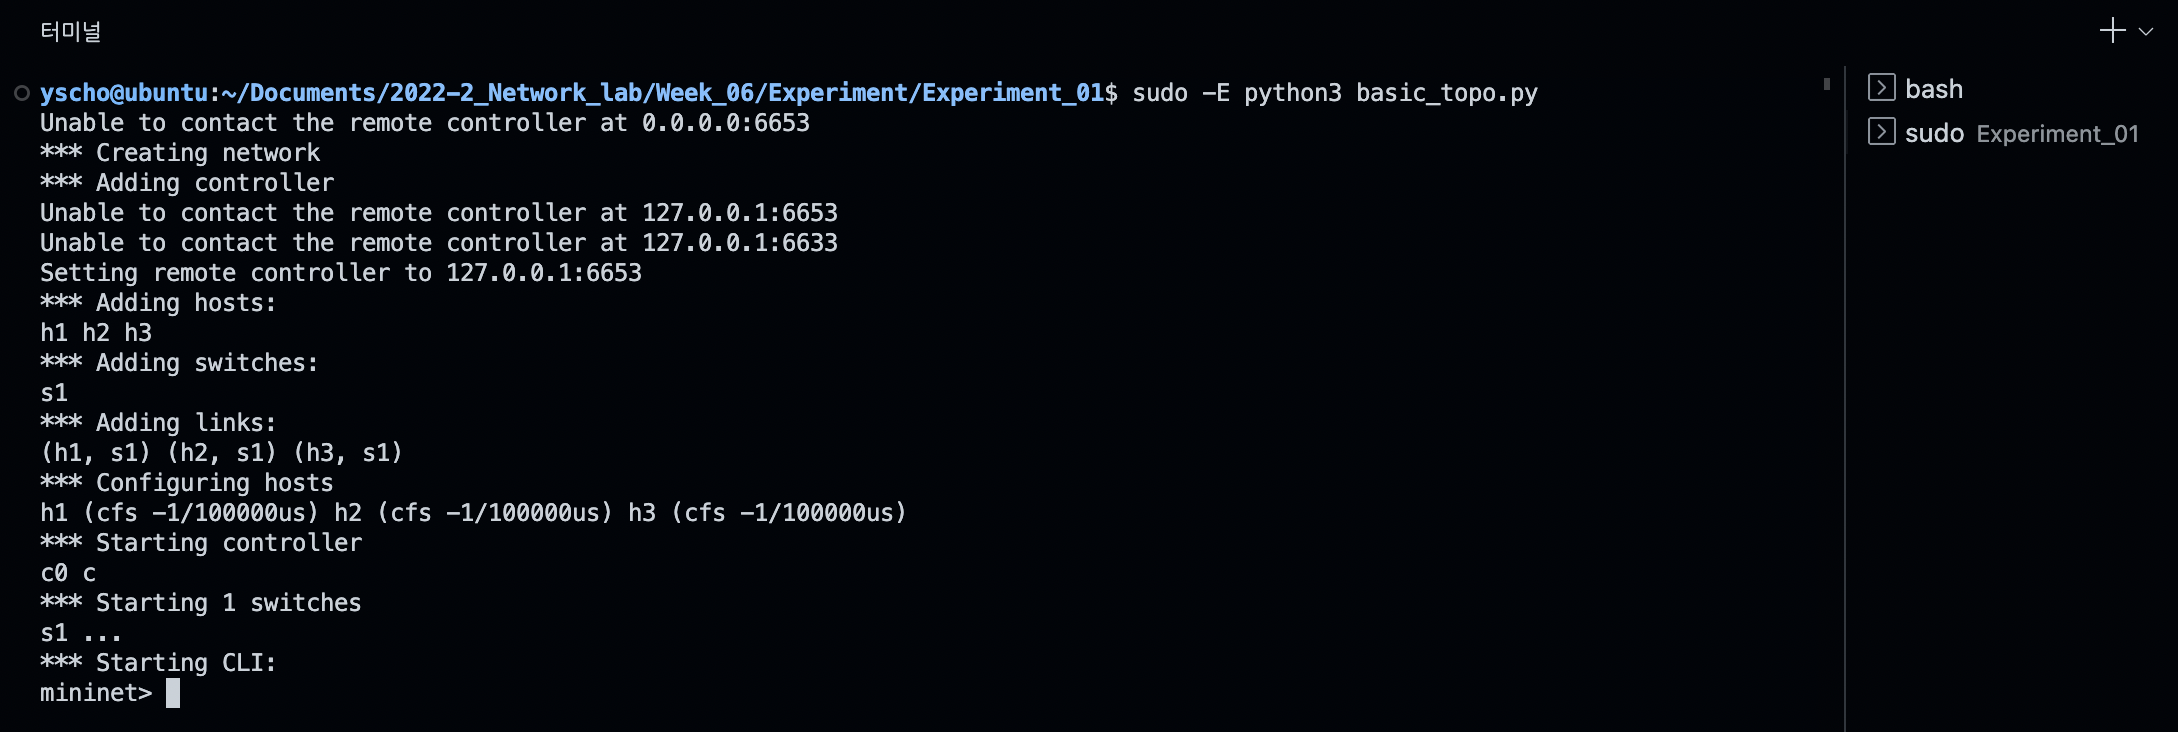
\includegraphics[width=.9\textwidth]{image/week06/1-3-2.png}
	\caption{\footnotesize 
	Terminal out screenshot : After executing the custom python topology code in bash terminal}
	\vspace{-10pt}
\end{figure}
\subsection*{4. Overview of Experiment 1, 2, 3}
In \textbf{Experiment 1}, we build a topology with 
\clearpage